\documentclass[12pt]{article}
\usepackage{amsmath}
\usepackage{graphicx}
\usepackage{hyperref}
\usepackage{geometry}
\geometry{margin=1in}
\usepackage{float}

\title{CTA200H Assignment 3}
\author{Zeinab Imani}
\date{}

\begin{document}

\maketitle

\section*{Question 1: Mandelbrot Set}

To explore the Mandelbrot set, we iterated the complex quadratic map:
$ z_{i+1} = z_i^2 + c, z_0 = 0 $
over the domain \( -2 < x < 2 \), \( -2 < y < 2 \), where \( c = x + iy \). A function was implemented in \texttt{function.py} to compute the number of iterations it took for the sequence to diverge, using an escape threshold of 10 and a maximum of 100 iterations.

Two plots were generated:
\begin{itemize}
    \item A binary image showing whether each point is bounded or diverges.
    \item A color-coded image showing how many iterations each point took to escape.
\end{itemize}

\begin{figure}[H]
    \centering
    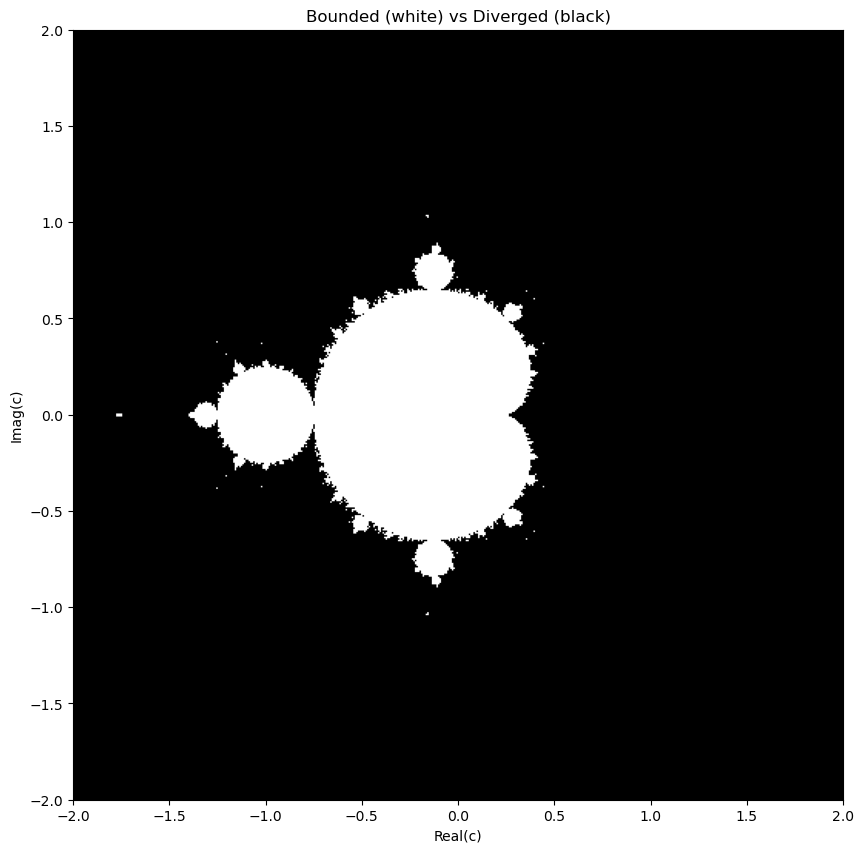
\includegraphics[width=0.65\textwidth]{download.png}
        \caption{Binary visualization: white = bounded, black = diverged.}
\end{figure}

\begin{figure}[H]
    \centering
    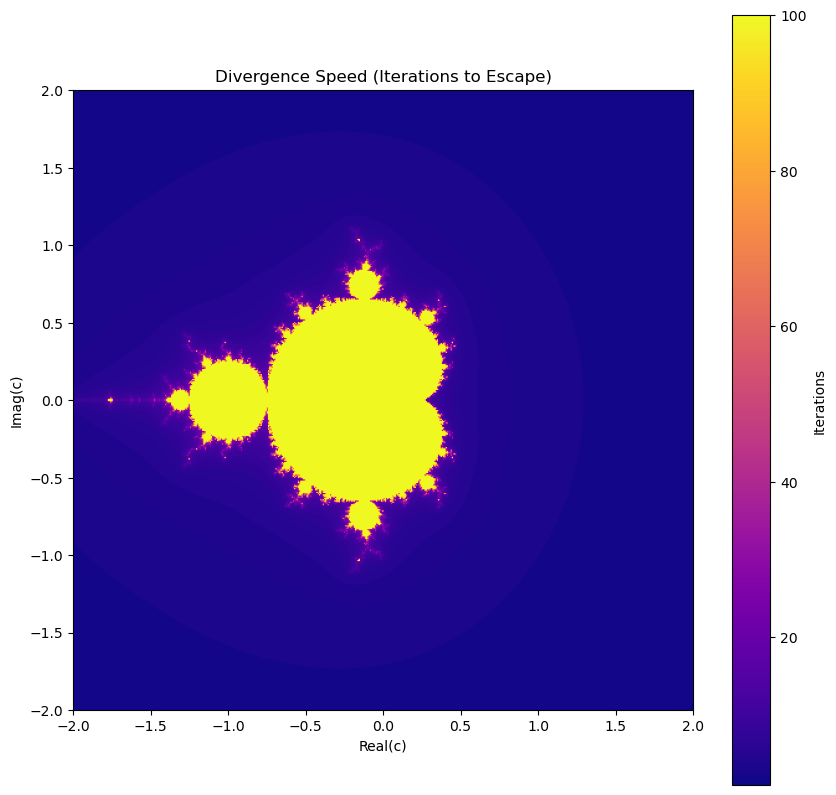
\includegraphics[width= 1 \textwidth]{download (1).png}
    \caption{Color map: divergence speed (number of iterations to escape).}
\end{figure}

\section*{Question 2: The Lorenz Attractor}

We numerically solved the Lorenz system:
\[
\begin{aligned}
\dot{X} &= \sigma(Y - X) \\
\dot{Y} &= rX - Y - XZ \\
\dot{Z} &= -bZ + XY
\end{aligned}
\]
with parameters \( \sigma = 10 \), \( r = 28 \), \( b = \frac{8}{3} \), and initial condition \( W_0 = [0, 1, 0] \), using \texttt{solve\_ivp}.

\subsection*{Figure 1: Y vs Time}
We plotted \( Y(t) \) over three intervals: t = 0–10, 10–20, and 20–30.

\begin{figure}[H]
    \centering
    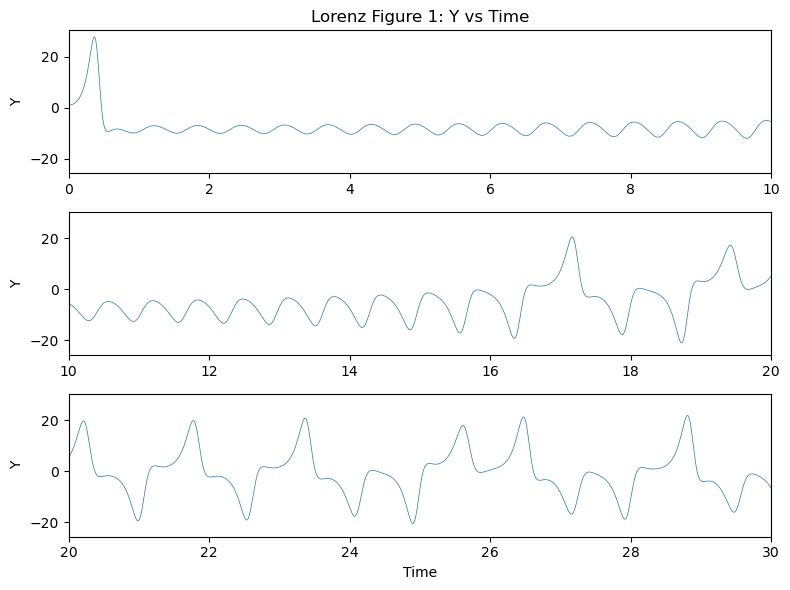
\includegraphics[width=1 \textwidth]{download (3).png}
    \caption{Lorenz Figure 1: Y vs Time over three 10-second segments.}
\end{figure}

\subsection*{Figure 2: Phase Space Projections}
We plotted:
\begin{itemize}
    \item Top: Z vs Y
    \item Bottom: Y vs X
\end{itemize}
for t in [14, 19], including markers labeled 14 to 19 at integer time steps.

\begin{figure}[H]
    \centering
    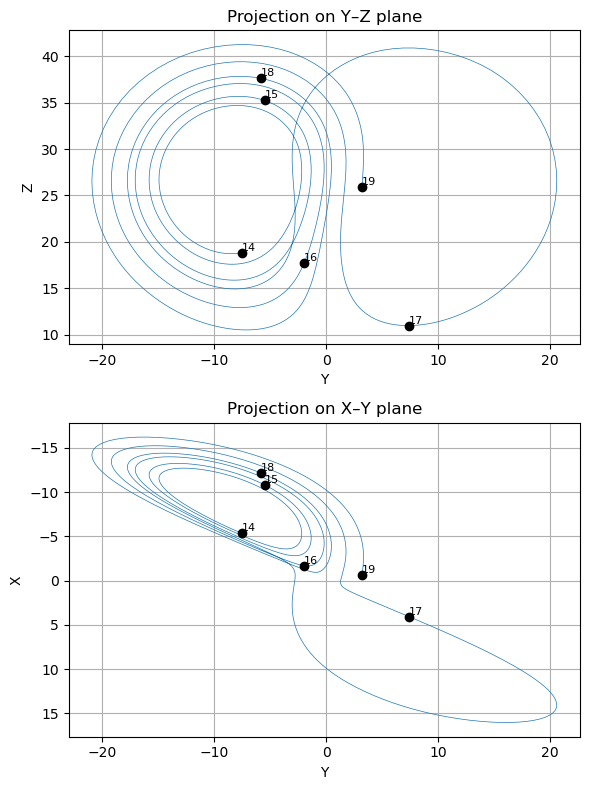
\includegraphics[width=0.8\textwidth]{download (4).png}
    \caption{Lorenz Figure 2: Phase projections with time labels.}
\end{figure}

\subsection*{Divergence from Nearby Initial Conditions}
We perturbed the initial condition by adding a small value to the second component:
\[
W_0' = W_0 + [0, 1 \times 10^{-8}, 0] = [0, 1.00000001, 0]
\]
We then solved the Lorenz equations again and computed the Euclidean distance between the two trajectories over time:
\[
d(t) = \left\| \mathbf{W}(t) - \mathbf{W}'(t) \right\|
\]
We plotted this distance on a semilog scale (logarithmic y-axis, linear x-axis). The nearly straight line confirms that the divergence grows exponentially—an important signature of chaotic behavior and sensitivity to initial conditions.

\begin{figure}[H]
    \centering
    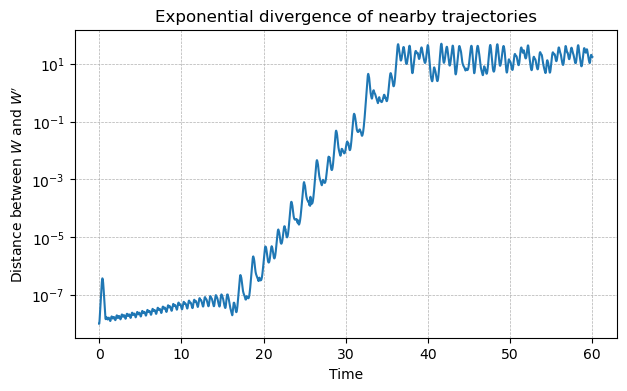
\includegraphics[width= 1 \textwidth]{download (2).png}
    \caption{Exponential divergence of nearby trajectories.}
\end{figure}

\clearpage



\end{document}
